\documentclass[crop=false]{standalone}
%\documentclass{standalone}
\usepackage{tikz} % To generate the plot from csv
\usepackage{pgfplots}
\usepackage{graphicx}
\usepackage{booktabs}
\usepackage{subfig}
\usepackage{float}
\usepackage[section]{placeins} % getting figures below sections
\usepackage{blindtext}
\usepackage{siunitx}
\usepgfplotslibrary{units} % Allows to enter the units nicely
\usetikzlibrary{external} %https://tex.stackexchange.com/questions/1460/script-to-automate-externalizing-tikz-graphics
\tikzexternalize[prefix=savedfigures/]

\pgfplotsset{compat=newest} % Allows to place the legend below plot
\usepackage{pgfplotstable}
\usepgfplotslibrary{statistics}

% #################### Function definition for box plots read table ##################\
\makeatletter
\pgfplotsset{
	boxplot prepared from table/.code={
		\def\tikz@plot@handler{\pgfplotsplothandlerboxplotprepared}%
		\pgfplotsset{
			/pgfplots/boxplot prepared from table/.cd,
			#1,
		}
	},
	/pgfplots/boxplot prepared from table/.cd,
	table/.code={\pgfplotstablecopy{#1}\to\boxplot@datatable},
	row/.initial=0,
	make style readable from table/.style={
		#1/.code={
			\pgfplotstablegetelem{\pgfkeysvalueof{/pgfplots/boxplot prepared from table/row}}{##1}\of\boxplot@datatable
			\pgfplotsset{boxplot/#1/.expand once={\pgfplotsretval}}
		}
	},
	make style readable from table=lower whisker,
	make style readable from table=upper whisker,
	make style readable from table=lower quartile,
	make style readable from table=upper quartile,
	make style readable from table=median,
	make style readable from table=average,
	make style readable from table=lower notch,
	make style readable from table=upper notch
}
\makeatother
\begin{document}

\section{3 1 Mandl6 GA Mutations 20210719 220507}

% ######################## UTRP GA Mutation operators applied ######################## 
\begin{figure} 
\centering 
\tikzsetnextfilename{UTRP_NSGAII_BP_mutation_funcs_phd} 
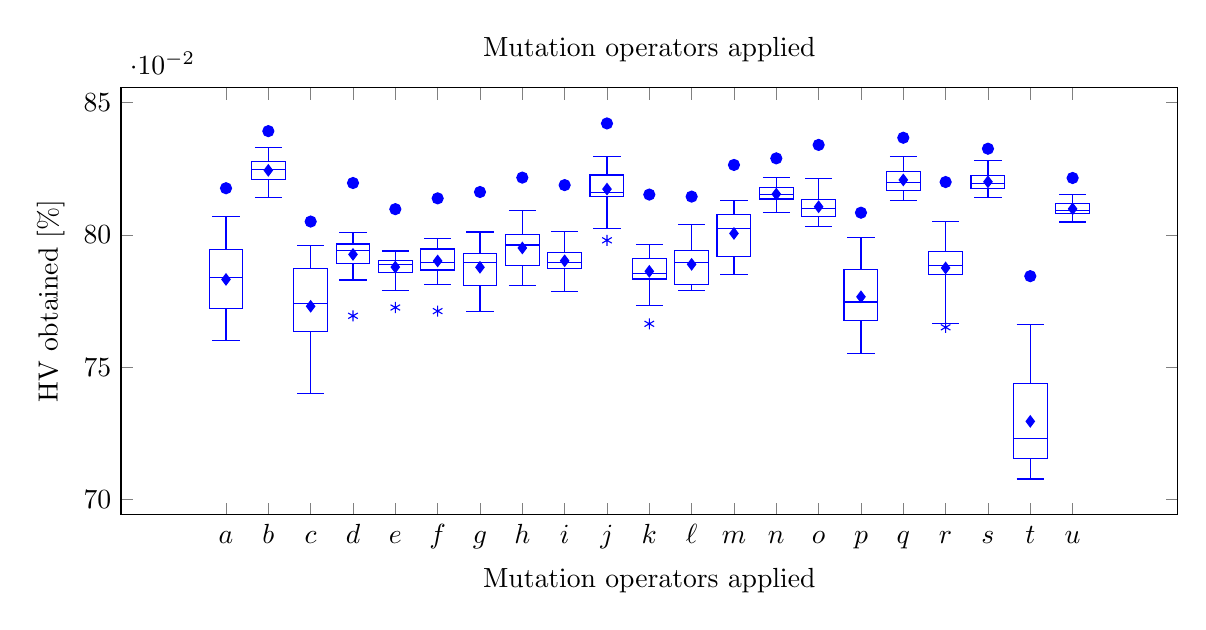
\begin{tikzpicture} 
\begin{axis}[ 
title={Mutation operators applied}, 
boxplot/draw direction=y, 
xtick={1,2,3,4,5,6,7,8,9,10,11,12,13,14,15,16,17,18,19,20,21}, 
%xticklabels={\vphantom{b}{a},\vphantom{b}{b},\vphantom{b}{c},d,\vphantom{b}{e},f,\vphantom{b}{g},h,\vphantom{b}{i},\vphantom{b}{j},k,l,\vphantom{b}{m},\vphantom{b}{n},\vphantom{b}{o},\vphantom{b}{p},\vphantom{b}{q},\vphantom{b}{r},\vphantom{b}{s},\vphantom{b}{t},\vphantom{b}{u}}, 
xticklabels={\vphantom{$b$}{$a$},\vphantom{$b$}{$b$},\vphantom{$b$}{$c$},$d$,\vphantom{$b$}{$e$},$f$,\vphantom{$b$}{$g$},$h$,\vphantom{$b$}{$i$},\vphantom{$b$}{$j$},$k$,$\ell$,\vphantom{$b$}{$m$},\vphantom{$b$}{$n$},\vphantom{$b$}{$o$},\vphantom{$b$}{$p$},\vphantom{$b$}{$q$},\vphantom{$b$}{$r$},\vphantom{$b$}{$s$},\vphantom{$b$}{$t$},\vphantom{$b$}{$u$}}, 
x tick label style={rotate=0, align=center}, 
xlabel={Mutation operators applied}, 
scaled y ticks={base 10:2}, %y tick label style={/pgf/number format/.cd,fixed,precision=3, zerofill}, 
ylabel={HV obtained [\%]}, 
height=7cm,
width=15cm
] 


% ############## Mutations=1 ################## 
\addplot[boxplot, mark=asterisk, 
boxplot prepared={ 
lower whisker=0.75992, 
upper whisker=0.80687, 
lower quartile=0.77204, 
upper quartile=0.79448, 
median=0.78397, 
average=0.78315}, 
color = blue, solid, area legend] 
coordinates {}; 
\addplot[only marks,mark=*,color = blue]coordinates{(1,0.81763)}; 

% ############## Mutations=2 ################## 
\addplot[boxplot, mark=asterisk, 
boxplot prepared={ 
lower whisker=0.81424, 
upper whisker=0.83313, 
lower quartile=0.82091, 
upper quartile=0.82782, 
median=0.82467, 
average=0.82439}, 
color = blue, solid, area legend] 
coordinates {}; 
\addplot[only marks,mark=*,color = blue]coordinates{(2,0.83921)}; 

% ############## Mutations=4 ################## 
\addplot[boxplot, mark=asterisk, 
boxplot prepared={ 
lower whisker=0.74014, 
upper whisker=0.79585, 
lower quartile=0.76342, 
upper quartile=0.78745, 
median=0.77418, 
average=0.773}, 
color = blue, solid, area legend] 
coordinates {}; 
\addplot[only marks,mark=*,color = blue]coordinates{(3,0.80503)}; 

% ############## Mutations=5 ################## 
\addplot[boxplot, mark=asterisk, 
boxplot prepared={ 
lower whisker=0.78295, 
upper whisker=0.80088, 
lower quartile=0.78913, 
upper quartile=0.79654, 
median=0.79394, 
average=0.7926}, 
color = blue, solid, area legend] 
coordinates {
(6,0.7694)}; 
\addplot[only marks,mark=*,color = blue]coordinates{(4,0.8196)}; 

% ############## Mutations=3 ################## 
\addplot[boxplot, mark=asterisk, 
boxplot prepared={ 
	lower whisker=0.77904, 
	upper whisker=0.7939, 
	lower quartile=0.78576, 
	upper quartile=0.79027, 
	median=0.7889, 
	average=0.78782}, 
color = blue, solid, area legend] 
coordinates {
	(4,0.77254)}; 
\addplot[only marks,mark=*,color = blue]coordinates{(5,0.80972)}; 

% ############## Mutations=6 ################## 
\addplot[boxplot, mark=asterisk, 
boxplot prepared={ 
lower whisker=0.78129, 
upper whisker=0.79877, 
lower quartile=0.7867, 
upper quartile=0.79466, 
median=0.78945, 
average=0.79013}, 
color = blue, solid, area legend] 
coordinates {
(7,0.77118)}; 
\addplot[only marks,mark=*,color = blue]coordinates{(6,0.8138)}; 

% ############## Mutations=7 ################## 
\addplot[boxplot, mark=asterisk, 
boxplot prepared={ 
lower whisker=0.77111, 
upper whisker=0.80107, 
lower quartile=0.78087, 
upper quartile=0.79282, 
median=0.78964, 
average=0.78774}, 
color = blue, solid, area legend] 
coordinates {}; 
\addplot[only marks,mark=*,color = blue]coordinates{(7,0.8162)}; 

% ############## Mutations=8 ################## 
\addplot[boxplot, mark=asterisk, 
boxplot prepared={ 
lower whisker=0.78084, 
upper whisker=0.80919, 
lower quartile=0.78852, 
upper quartile=0.79997, 
median=0.79617, 
average=0.79505}, 
color = blue, solid, area legend] 
coordinates {}; 
\addplot[only marks,mark=*,color = blue]coordinates{(8,0.82164)}; 

% ############## Mutations=9 ################## 
\addplot[boxplot, mark=asterisk, 
boxplot prepared={ 
lower whisker=0.77858, 
upper whisker=0.80129, 
lower quartile=0.78715, 
upper quartile=0.79336, 
median=0.78946, 
average=0.79021}, 
color = blue, solid, area legend] 
coordinates {}; 
\addplot[only marks,mark=*,color = blue]coordinates{(9,0.81881)}; 

% ############## Mutations=0 ################## 
\addplot[boxplot, mark=asterisk, 
boxplot prepared={ 
	lower whisker=0.80248, 
	upper whisker=0.82976, 
	lower quartile=0.81451, 
	upper quartile=0.82264, 
	median=0.81617, 
	average=0.8173}, 
color = blue, solid, area legend] 
coordinates {
	(1,0.79794)}; 
\addplot[only marks,mark=*,color = blue]coordinates{(10,0.84212)}; 

% ############## Mutations=10 ################## 
\addplot[boxplot, mark=asterisk, 
boxplot prepared={ 
lower whisker=0.77341, 
upper whisker=0.7965, 
lower quartile=0.78332, 
upper quartile=0.79104, 
median=0.78552, 
average=0.7862}, 
color = blue, solid, area legend] 
coordinates {
(11,0.76638)}; 
\addplot[only marks,mark=*,color = blue]coordinates{(11,0.81523)}; 

% ############## Mutations=11 ################## 
\addplot[boxplot, mark=asterisk, 
boxplot prepared={ 
lower whisker=0.77904, 
upper whisker=0.80392, 
lower quartile=0.78131, 
upper quartile=0.79418, 
median=0.78964, 
average=0.78886}, 
color = blue, solid, area legend] 
coordinates {}; 
\addplot[only marks,mark=*,color = blue]coordinates{(12,0.81446)}; 

% ############## Mutations=14 ################## 
\addplot[boxplot, mark=asterisk, 
boxplot prepared={ 
lower whisker=0.7849, 
upper whisker=0.81294, 
lower quartile=0.79194, 
upper quartile=0.80781, 
median=0.80252, 
average=0.80054}, 
color = blue, solid, area legend] 
coordinates {}; 
\addplot[only marks,mark=*,color = blue]coordinates{(13,0.82643)}; 

% ############## Mutations=12 ################## 
\addplot[boxplot, mark=asterisk, 
boxplot prepared={ 
	lower whisker=0.80845, 
	upper whisker=0.82168, 
	lower quartile=0.81357, 
	upper quartile=0.81791, 
	median=0.81533, 
	average=0.81541}, 
color = blue, solid, area legend] 
coordinates {}; 
\addplot[only marks,mark=*,color = blue]coordinates{(14,0.82892)}; 

% ############## Mutations=13 ################## 
\addplot[boxplot, mark=asterisk, 
boxplot prepared={ 
	lower whisker=0.80321, 
	upper whisker=0.82142, 
	lower quartile=0.807, 
	upper quartile=0.8135, 
	median=0.80997, 
	average=0.81063}, 
color = blue, solid, area legend] 
coordinates {}; 
\addplot[only marks,mark=*,color = blue]coordinates{(15,0.834)}; 

% ############## Mutations=18 ################## 
\addplot[boxplot, mark=asterisk, 
boxplot prepared={ 
	lower whisker=0.75517, 
	upper whisker=0.79905, 
	lower quartile=0.76774, 
	upper quartile=0.78701, 
	median=0.77463, 
	average=0.77658}, 
color = blue, solid, area legend] 
coordinates {}; 
\addplot[only marks,mark=*,color = blue]coordinates{(16,0.80838)};

% ############## Mutations=15 ################## 
\addplot[boxplot, mark=asterisk, 
boxplot prepared={ 
lower whisker=0.81298, 
upper whisker=0.82962, 
lower quartile=0.81682, 
upper quartile=0.82392, 
median=0.81975, 
average=0.82077}, 
color = blue, solid, area legend] 
coordinates {}; 
\addplot[only marks,mark=*,color = blue]coordinates{(17,0.83671)}; 

% ############## Mutations=19 ################## 
\addplot[boxplot, mark=asterisk, 
boxplot prepared={ 
	lower whisker=0.76643, 
	upper whisker=0.80509, 
	lower quartile=0.78487, 
	upper quartile=0.79364, 
	median=0.78841, 
	average=0.7875}, 
color = blue, solid, area legend] 
coordinates {
	(20,0.76505)}; 
\addplot[only marks,mark=*,color = blue]coordinates{(18,0.81997)}; 

% ############## Mutations=16 ################## 
\addplot[boxplot, mark=asterisk, 
boxplot prepared={ 
lower whisker=0.81412, 
upper whisker=0.82826, 
lower quartile=0.81746, 
upper quartile=0.8224, 
median=0.81928, 
average=0.82006}, 
color = blue, solid, area legend] 
coordinates {}; 
\addplot[only marks,mark=*,color = blue]coordinates{(19,0.83256)}; 

% ############## Mutations=20 ################## 
\addplot[boxplot, mark=asterisk, 
boxplot prepared={ 
lower whisker=0.70773, 
upper whisker=0.76608, 
lower quartile=0.71544, 
upper quartile=0.74386, 
median=0.72289, 
average=0.7295}, 
color = blue, solid, area legend] 
coordinates {}; 
\addplot[only marks,mark=*,color = blue]coordinates{(20,0.78439)}; 

% ############## Mutations=17 ################## 
\addplot[boxplot, mark=asterisk, 
boxplot prepared={ 
	lower whisker=0.80485, 
	upper whisker=0.81529, 
	lower quartile=0.80809, 
	upper quartile=0.81179, 
	median=0.80922, 
	average=0.80985}, 
color = blue, solid, area legend] 
coordinates {}; 
\addplot[only marks,mark=*,color = blue]coordinates{(21,0.8215)}; 

\end{axis}
\end{tikzpicture}
\end{figure} 
\begin{table}
\centering
\caption{Legend for the boxplot.}
\begin{tabular}{ll}
\toprule
 Index &                      Name \\
\midrule
     0 &          [Intertwine\_two] \\
     1 &              [Add\_vertex] \\
     2 &           [Delete\_vertex] \\
     3 &    [Invert\_path\_vertices] \\
     4 &    [Insert\_inside\_vertex] \\
     5 &    [Delete\_inside\_vertex] \\
     6 &  [Relocate\_inside\_vertex] \\
     7 &   [Replace\_inside\_vertex] \\
     8 &   [Donate\_between\_routes] \\
     9 &     [Swap\_between\_routes] \\
    10 &         [Merge\_terminals] \\
    11 &      [Repl\_low\_dem\_route] \\
    12 &    [Rem\_low\_dem\_terminal] \\
    13 &   [Rem\_lrg\_cost\_terminal] \\
    14 &            [Repl\_subsets] \\
    15 &    [Trim\_one\_terminal\_cb] \\
    16 & [Trim\_one\_path\_random\_cb] \\
    17 &   [Trim\_routes\_random\_cb] \\
    18 &    [Grow\_one\_terminal\_cb] \\
    19 & [Grow\_one\_path\_random\_cb] \\
    20 &   [Grow\_routes\_random\_cb] \\
\bottomrule
\end{tabular}
\end{table}

\begin{table}
	\centering
	\caption{Legend for the boxplot.}
	\begin{tabular}{ll}
		\toprule
		Index &                      Name \\
		\midrule
		1 &              [Add\_vertex] \\
		2 &           [Delete\_vertex] \\
		4 &    [Insert\_inside\_vertex] \\
		5 &    [Delete\_inside\_vertex] \\
		3 &    [Invert\_path\_vertices] \\
		6 &  [Relocate\_inside\_vertex] \\
		7 &   [Replace\_inside\_vertex] \\
		8 &   [Donate\_between\_routes] \\
		9 &     [Swap\_between\_routes] \\
		0 &          [Intertwine\_two] \\
		10 &         [Merge\_terminals] \\
		11 &      [Repl\_low\_dem\_route] \\
		14 &            [Repl\_subsets] \\
		12 &    [Rem\_low\_dem\_terminal] \\
		13 &   [Rem\_lrg\_cost\_terminal] \\
		18 &    [Grow\_one\_terminal\_cb] \\
		15 &    [Trim\_one\_terminal\_cb] \\
		19 & [Grow\_one\_path\_random\_cb] \\
		16 & [Trim\_one\_path\_random\_cb] \\
		20 &   [Grow\_routes\_random\_cb] \\
		17 &   [Trim\_routes\_random\_cb] \\
		\bottomrule
	\end{tabular}
\end{table}


\begin{table}
	\centering
	\caption{Coordinate conversion.}
	\begin{tabular}{rll}
		\toprule
		From & To & Adjustment\\
		\midrule
1  & 0  & $+1$\\
2  & 1  & $+1$\\
4  & 2  & $+1$\\
5  & 3  & $+1$\\
3  & 4  & $+1$\\
6  & 5  & $+1$\\
7  & 6  & $+1$\\
8  & 7  & $+1$\\
9  & 8  & $+1$\\
0  & 9  & $+1$\\
10 & 10 & $+1$\\
11 & 11 & $+1$\\
14 & 12 & $+1$\\
12 & 13 & $+1$\\
13 & 14 & $+1$\\
18 & 15 & $+1$\\
15 & 16 & $+1$\\
19 & 17 & $+1$\\
16 & 18 & $+1$\\
20 & 19 & $+1$\\
17 & 20 & $+1$\\
		\bottomrule
	\end{tabular}
\end{table}

\end{document}